\chapter{System Analysis and Design}
\label{chap:system_analysis}

\section{Introduction}
\label{sec:sys_intro}
This chapter provides a comprehensive analysis of the educational platform's architecture, detailing its structural components, data flow, and user interactions. Through various modeling techniques, we break down the system's core functionalities and processes to ensure a robust foundation for implementation. The analysis employs multiple diagrammatic approaches to illustrate different perspectives of the system, from high-level ecosystem interactions to detailed process workflows. The analytical framework includes:
\begin{itemize}
    \item \textbf{Context Diagram:} Presenting the platform's ecosystem and its interactions with external entities and user roles.
    \item \textbf{Data Flow Diagram (DFD):} Illustrating the movement and transformation of data across system processes.
    \item \textbf{Activity Diagrams:} Modeling the progression of business processes and user workflows within the platform.
    \item \textbf{Class Diagram:} Defining the static structure of the system through entities, their attributes, and relationships.
    \item \textbf{Sequence Diagram:} Depicting the chronological flow of interactions between system components and external services.
    \item \textbf{Use Case Diagram:} Offering a high-level representation of system functionalities and interactions between actors.
    \item \textbf{Use Case Analysis:} Providing a detailed examination of use case steps, actors, and conditions.
\end{itemize}
Collectively, these diagrams establish a clear blueprint for system development, ensuring all functional requirements are properly addressed while maintaining scalability and user experience excellence.

\section{System Requirements}
\label{sec:system_reqs}
This section outlines the core functional and non-functional requirements for the educational platform.

\subsection{Functional Requirements}
\label{subsec:func_reqs}
\begin{itemize}
    \item Users can register, log in, and manage their profiles with role-based access (Student, Mentor, Admin).
    \item Students can browse courses, enroll in available courses, and access learning materials (videos, PDFs, problem sets).
    \item The system supports submission of solutions to problems, with automatic evaluation and verdict delivery.
    \item Mentors can create and manage course content, monitor student progress, and facilitate group interactions.
    \item Admins can manage users, assign roles, oversee site settings, and generate system-wide reports.
    \item The platform provides personalized learning recommendations based on student performance and progress analytics.
    \item The system integrates with external judges for real-time code evaluation and plagiarism detection.
\end{itemize}

\subsection{Non-Functional Requirements}
\label{subsec:non_func_reqs}
\begin{itemize}
    \item The system must implement robust data encryption for all sensitive user information, particularly national and college IDs, ensuring secure storage and transmission.
    \item Access control must be enforced through role-based permissions for administrative dashboards, utilizing JWT tokens and HTTPS for secure API communication.
    \item The platform must maintain high availability through asynchronous processing for code evaluation and real-time features like chat and notifications.
    \item System performance must be monitored through key metrics including user engagement, submission pass rates, and course completion rates.
    \item Multi-channel notifications must be implemented for critical alerts, distributed via in-app messages, email, and integrated platforms like Discord and Telegram.
    \item The architecture must support horizontal scaling to accommodate growing user loads while maintaining response times under 2 seconds for core features.
    \item The platform must implement automated spam detection and rate limiting to ensure system stability and prevent resource exhaustion.
\end{itemize}

\section{Context Diagram}
\label{sec:context_diagram}
The context diagram provides the highest-level view of the E-Learning platform, representing it as a single process and illustrating its interactions with all major external entities.

\begin{figure}[h!]
    \centering
    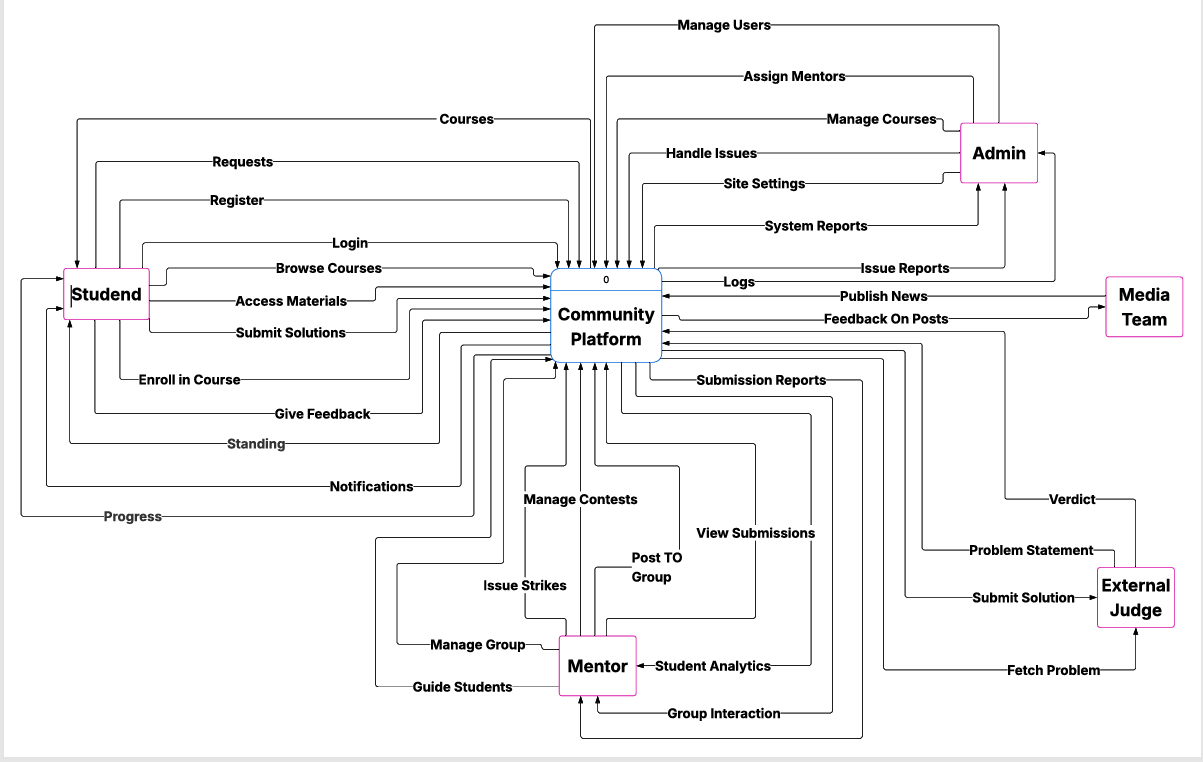
\includegraphics[width=\textwidth]{figures/chapter4/context_diagram.png}
    \caption{System Context Diagram.}
    \label{fig:context_diagram}
\end{figure}

\section{Data Flow Diagram}
\label{sec:dfd}
A Data Flow Diagram (DFD) illustrates how the E-Linker platform processes information, focusing on the movement of data between processes, external entities, and data stores. It provides a clear overview of how data is transformed, where it is stored, and how it flows through the system to support various educational functions.

\begin{figure}[h!]
    \centering
    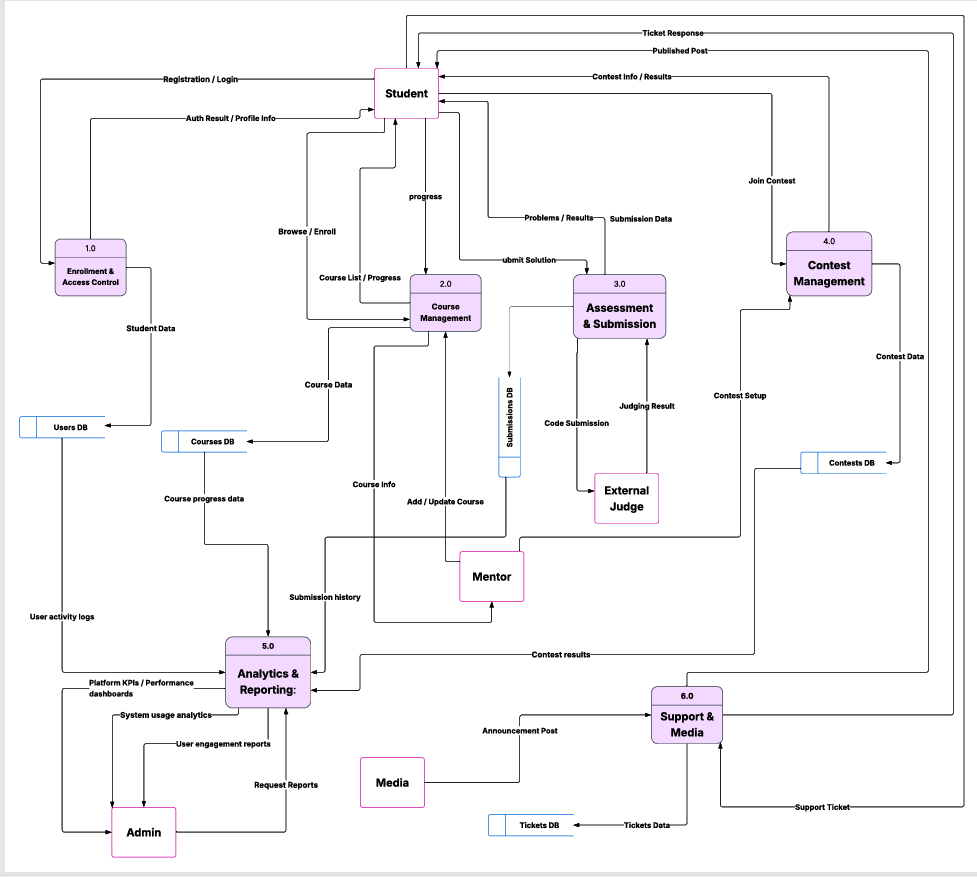
\includegraphics[width=\textwidth]{figures/chapter4/dfd.png}
    \caption{Level 1 Data Flow Diagram (DFD).}
    \label{fig:dfd}
\end{figure}

\section{Use Case Diagram}
\label{sec:use_case_diagram}
The Use Case Diagram provides a complete visual representation of the system's functional scope and all authorized interactions for each primary actor. A use case diagram illustrates the platform's functionality from the user's perspective. It identifies all system users and demonstrates how they interact with the platform. The diagram visualizes relationships between different use cases and actors. It defines the boundary between the system and its external environment.

\begin{figure}[h!]
    \centering
    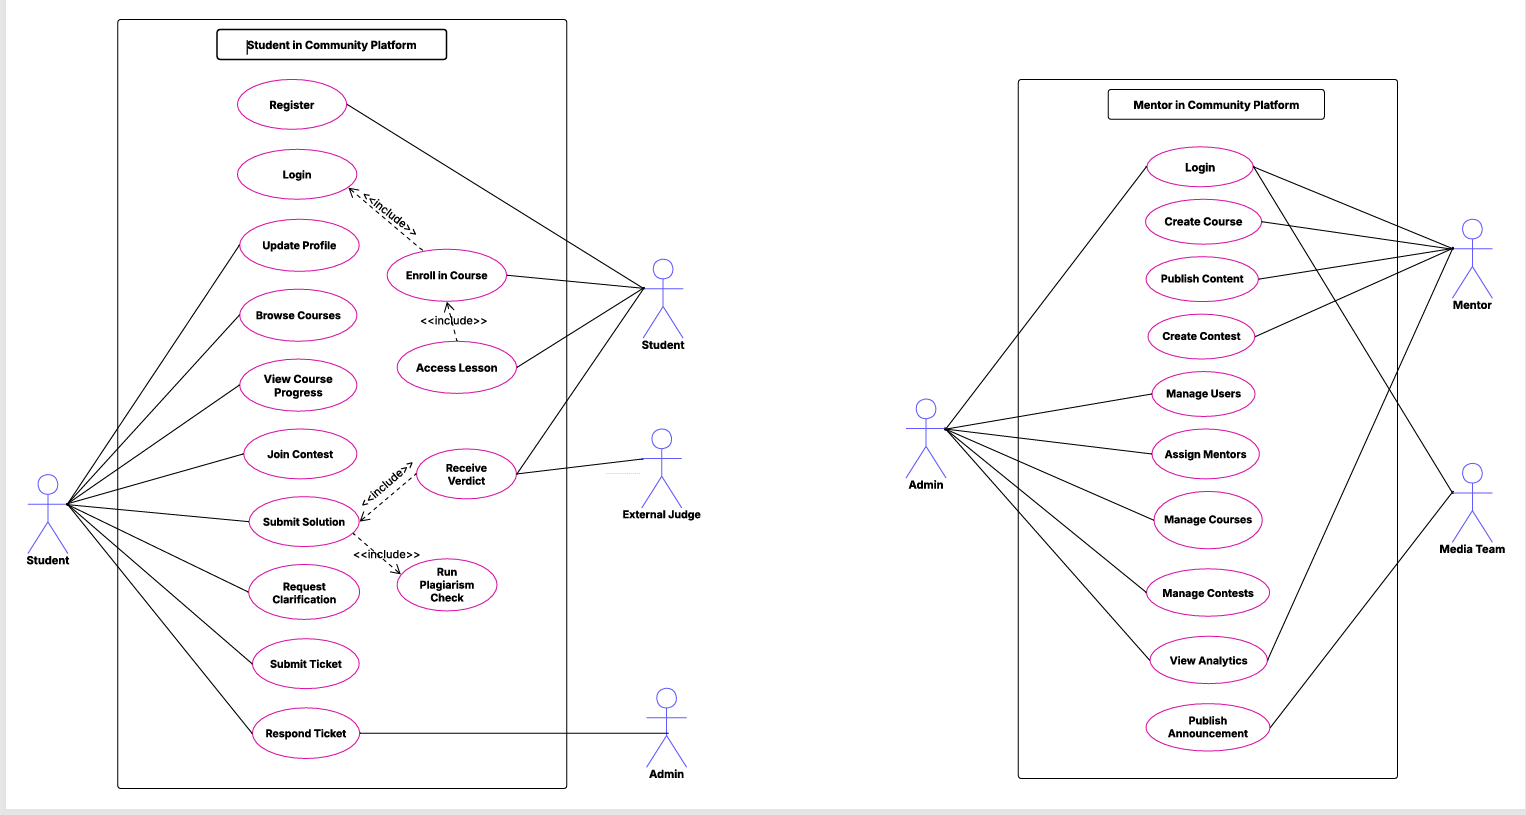
\includegraphics[width=\textwidth]{figures/chapter4/use_case_diagram.png}
    \caption{System Use Case Diagram.}
    \label{fig:use_case_diagram}
\end{figure}

\section{Use Case Scenarios: Detailed System Flows}
\label{sec:use_case_scenarios}
Detailed scenarios define the step-by-step interactions for core, complex, and specialized system processes.

\subsection{UC 1: User Registration and Identity Verification}
\label{subsec:uc1}
This scenario details the complete workflow for new user onboarding, incorporating multi-level verification to ensure platform integrity and compliance.
\begin{enumerate}
    \item \textbf{Student} navigates to the registration page and provides essential credentials: username, full name, email, and password.
    \item Optionally submits verification documents: phone number, college ID, or national ID.
    \item \textbf{System} performs real-time validation checking for duplicate usernames/emails and data format compliance.
    \item \textbf{Decision Point (Validation):}
    \begin{itemize}
        \item If Validation Fails: System returns specific field-level error messages with correction guidance.
        \item If Validation Succeeds: System creates a temporary account with "pending verification" status and dispatches a verification email with a time-sensitive activation link.
    \end{itemize}
    \item For ID submissions: \textbf{System} routes documents to an encrypted Reviewer Dashboard queue for manual verification.
    \item \textbf{Reviewer} conducts manual verification comparing submitted documents against user profile data.
    \item \textbf{Decision Point (Verification Level):}
    \begin{itemize}
        \item Basic Verification (email only): Grants access to public courses and community features.
        \item Enhanced Verification (ID approved): Unlocks exam participation, contest access, and premium content.
    \end{itemize}
    \item \textbf{System} notifies the user of verification status and corresponding access privileges, generating a comprehensive audit trail of registration events.
\end{enumerate}

\subsection{UC 2 (Synthetic): Secure Exam Initiation and Proctoring}
\label{subsec:uc2}
This scenario illustrates the multi-layered process for deploying high-integrity online exams, combining system controls and AI monitoring.
\begin{enumerate}
    \item \textbf{Student} navigates to the exam page and clicks 'Start Secure Exam'.
    \item \textbf{System} validates the student's environment by utilizing the JavaScript Visibility API to check for multiple open browser tabs or windows, blocking the start if unauthorized activity is detected.
    \item \textbf{System} requests and verifies access to the student's Webcam and Microphone, initializing the Computer Vision components (OpenCV/MediaPipe).
    \item \textbf{System} programmatically activates anti-cheating controls, specifically disabling native browser functions for copy/paste and preventing screen capture.
    \item \textbf{Secure Exam Module} loads the exam content, ensuring it is decrypted only upon start and held in a protected local storage mechanism (Secure Caching/Encrypted IndexedDB) to prevent content leakage.
    \item The \textbf{AI/CV Monitoring Service} begins real-time streaming and analysis of video/audio data, actively searching for behavioral anomalies that indicate cheating (e.g., unusual head movements, detection of a second person).
    \item \textbf{Student} is presented with the exam content and begins the assessment under continuous surveillance.
\end{enumerate}

\subsection{UC 3 (Synthetic): Personalized Question Recommendation}
\label{subsec:uc3}
This flow describes the data pipeline that powers the adaptive learning system.
\begin{enumerate}
    \item \textbf{Student} navigates to the course practice area and selects 'Get Personalized Practice'.
    \item \textbf{Core System} queries the Analytics DB (DFD Process 5.0) to retrieve the Student’s complete performance metrics, including their current level, recent assessment scores, and detailed submission history.
    \item The relevant data subset is transmitted to the dedicated \textbf{ML Recommendation Service} (running Python + scikit-learn).
    \item The \textbf{ML Service} processes the student’s profile against its models, using performance metrics (e.g., time-to-solve, tags of incorrectly answered questions) to generate a set of optimal Question IDs, potentially leveraging ML embeddings for precision.
    \item The \textbf{ML Service} returns the prioritized list of recommended Question IDs to the Core System.
    \item \textbf{Core System} retrieves the full problem statements and associated metadata for the recommended questions from the database.
    \item \textbf{Student} receives the practice set, which is dynamically tailored to address their specific identified knowledge gaps and weaknesses.
\end{enumerate}

\section{Activity Diagrams}
\label{sec:activity_diagrams}
Activity diagrams model the processes required to execute key functionalities, highlighting branching and parallel execution.

\begin{figure}[h!]
    \centering
    
    \begin{subfigure}[b]{0.45\textwidth}
        \centering
        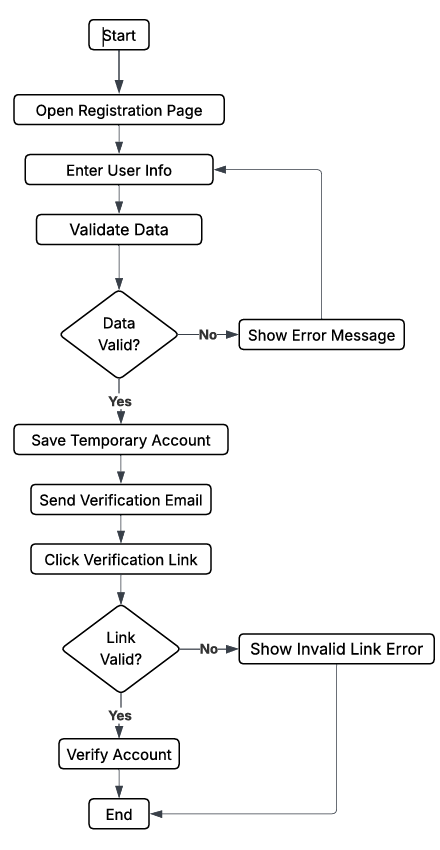
\includegraphics[width=\textwidth]{figures/chapter4/activity_registration.png}
        \caption{User Registration.}
        \label{fig:activity_registration}
    \end{subfigure}
    \hfill 
    \begin{subfigure}[b]{0.45\textwidth}
        \centering
        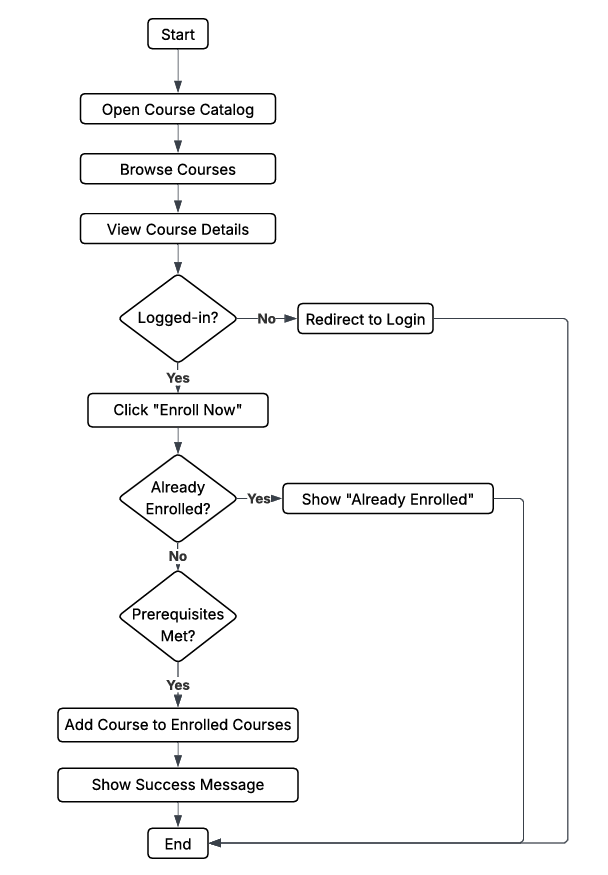
\includegraphics[width=\textwidth]{figures/chapter4/activity_enrollment.png}
        \caption{Course Enrollment.}
        \label{fig:activity_enrollment}
    \end{subfigure}
    
    \caption{Activity Diagrams for User Onboarding and Enrollment.}
    \label{fig:user_activity_diagrams}
\end{figure}

\begin{figure}[h!]
    \centering
    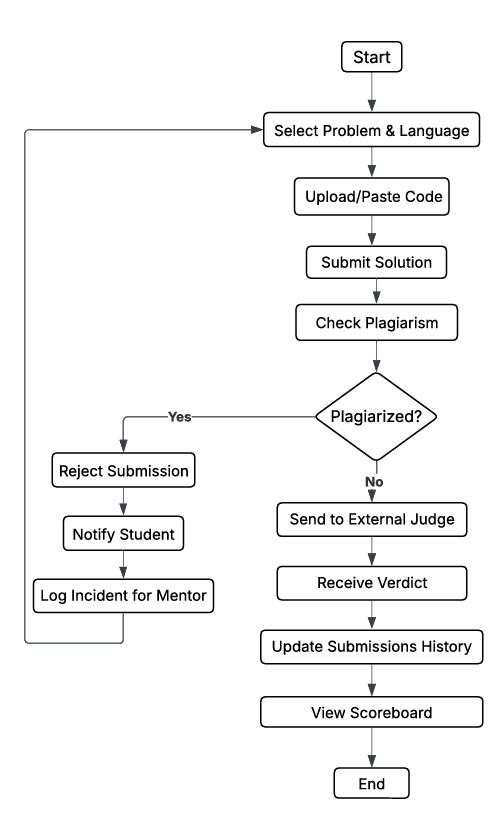
\includegraphics[width=0.5\textwidth]{figures/chapter4/activity_submission.png}
    \caption{Activity Diagram for Code Submission.}
    \label{fig:activity_submission}
\end{figure}


\section{Sequence Diagram}
\label{sec:sequence_diagram}
Sequence Diagrams illustrate the dynamic interaction and message passing between system components, confirming the operational feasibility of decoupled and specialized features.

\begin{figure}[h!]
    \centering
    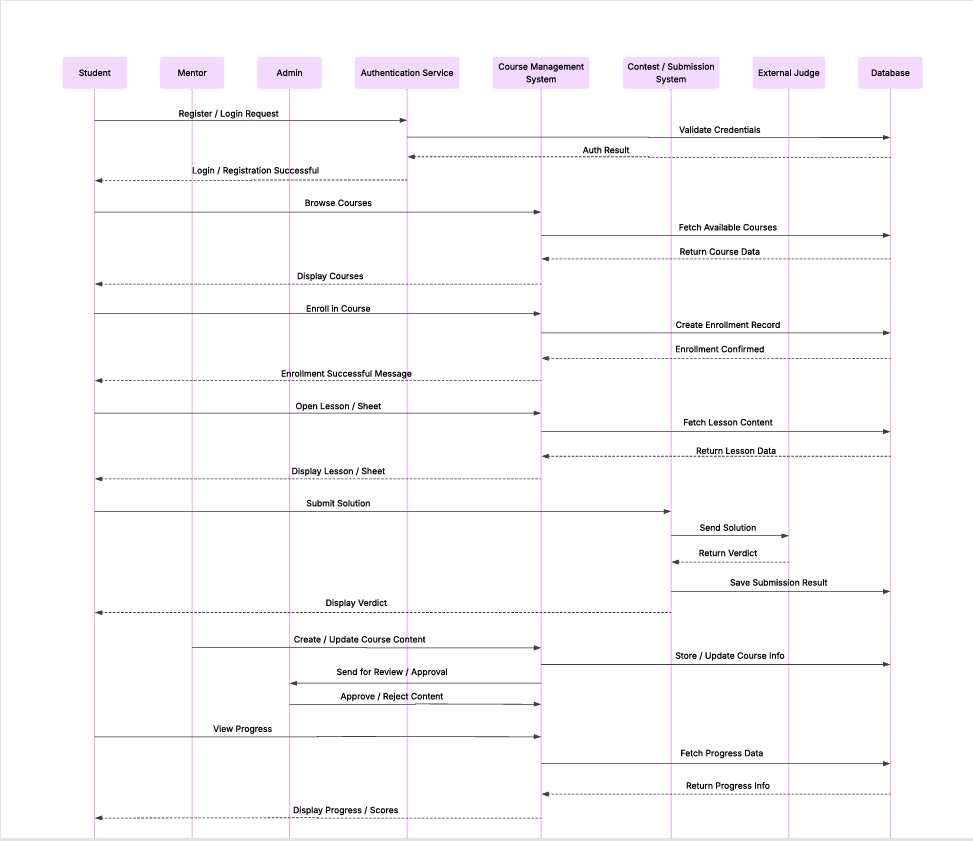
\includegraphics[width=\textwidth]{figures/chapter4/sequence_diagram.png}
    \caption{System Sequence Diagram.}
    \label{fig:sequence_diagram}
\end{figure}

\section{Class Diagram}
\label{sec:class_diagram}
The Class Diagram defines the definitive static structure of the E-learning system, detailing specialized classes and their encapsulated operations, directly implementing the platform's unique requirements.

\begin{figure}[h!]
    \centering
    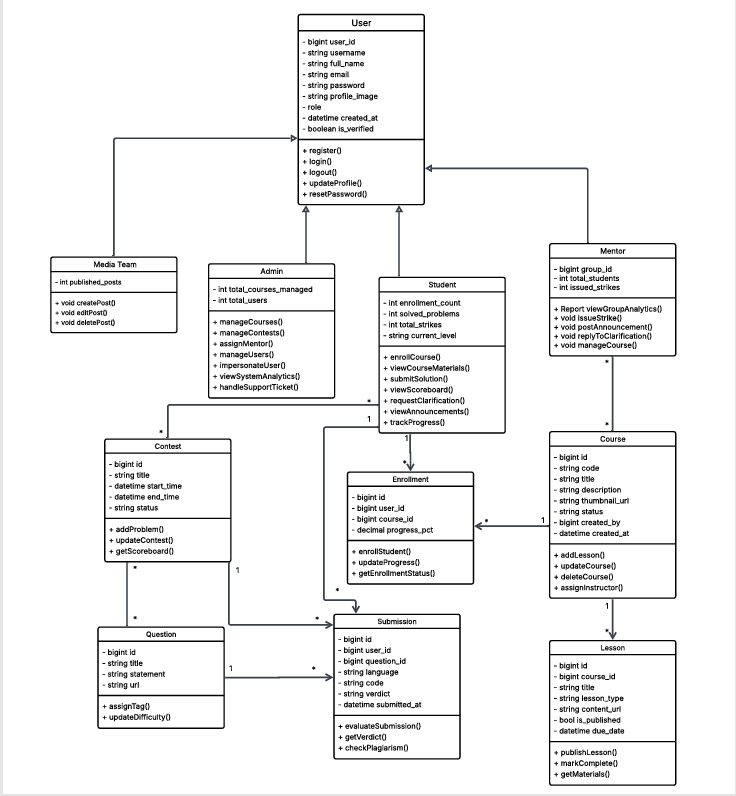
\includegraphics[width=\textwidth]{figures/chapter4/class_diagram.png}
    \caption{System Class Diagram.}
    \label{fig:class_diagram}
\end{figure}